% Reviewed fixed result figure; public renderer stages candidates separately.
\begin{figure}[t]
\centering
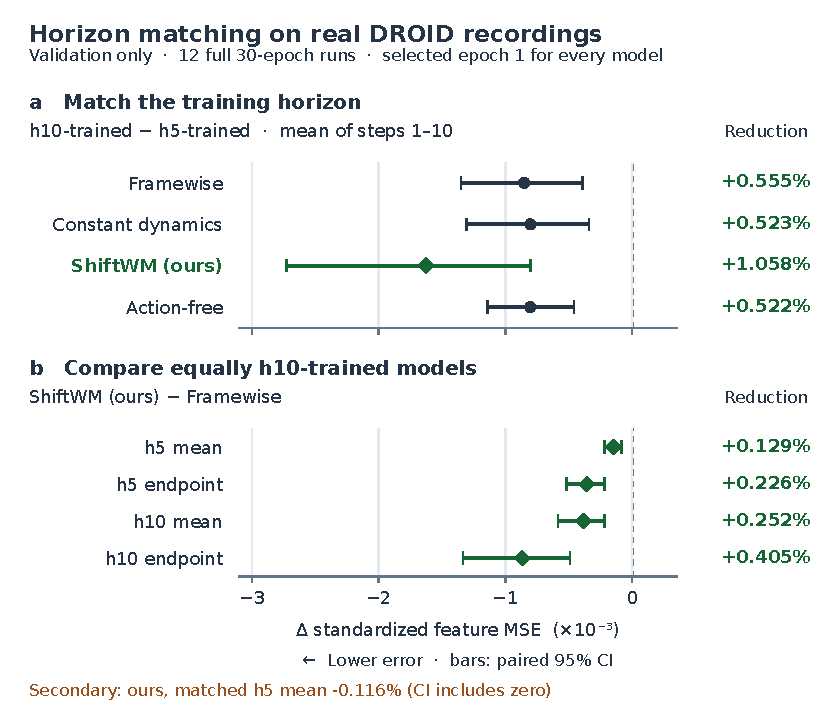
\includegraphics[width=\textwidth]{generated/real_video/horizon10_summary.pdf}
\caption[Horizon matching on real DROID recordings.]{Horizon matching on real DROID recordings (original validation only). (a) For each unchanged mode, h10-trained minus original h5-trained standardized feature MSE, averaged over steps 1--10 on identical h10-eligible windows. Training and checkpoint-selection horizons change together. (b) ShiftWM (ours; factorized) minus equally h10-trained Framewise, for all-query mean and endpoint errors at h5 and h10. Dots and bars show signed MSE differences and paired 95\% recording-session $\times$ training-seed bootstrap intervals (10,000 draws; seed 5198010). Negative differences favor the first model. Bold green percentages are relative point reductions, not confidence intervals. Both panels use the same absolute-error axis. There are 141 eligible episodes from 59 sessions and 3 model seeds; standard h5 has 1,772 windows, while h10 and matched h5 prefixes have 1,631. Windows are averaged within episodes, then episodes and seeds equally. All 12 runs completed 30 epochs; all selected epoch 1 by the fixed window-weighted validation criterion. The unfavorable secondary matched h5-prefix mean for factorized is -0.116\% relative reduction, a small increase in error; new-minus-original MSE difference +0.0001264, paired 95\% CI [-0.0002152, +0.0005941]. All 20 registered contrasts are retained in the companion evidence ledger. These are exploratory, multiplicity-unadjusted validation comparisons, not independent test or state-of-the-art claims.}
\label{fig:horizon10_summary}
\end{figure}
